\section{Noise.}
\begin{enumerate}[label=\emph{\alph*)}]
\item Take the original colored image (img) and add Gaussian noise to the pixels in the green channel. Increase the sigma until the noise is visible in the image. Store the image into the output folder. What is the value of sigma you used? How did the noise in the resulting images behave? What did you observe?

The results of adding gaussian noise to the blue channel are shown in figure \ref{fig:gaussian-noise-green}. The value of sigma used is 30, the noise tends to affect black/white-like areas, this is more clean in figures \ref{fig:gaussian-noise-green}.b and \ref{fig:gaussian-noise-green}.d, the noise does affect selective parts of the image.

\begin{figure}[h!]
\centering
  \begin{subfigure}{0.5\textwidth}
    \centering
    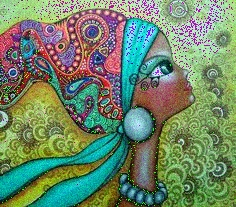
\includegraphics[width=0.5\linewidth]{../output/p0-5-a-0.jpg}
    \caption{Gaussian noise on p0-1-0.jpg green channel}
  \end{subfigure}%
\begin{subfigure}{0.5\textwidth}
  \centering
  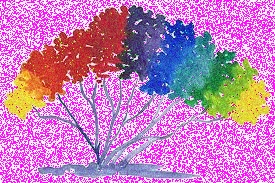
\includegraphics[width=0.5\linewidth]{../output/p0-5-a-1.jpg}
  \caption{Gaussian noise on p0-1-1.jpg green channel}
  \label{fig:sfig2}
\end{subfigure}
\begin{subfigure}{0.5\textwidth}
  \centering
  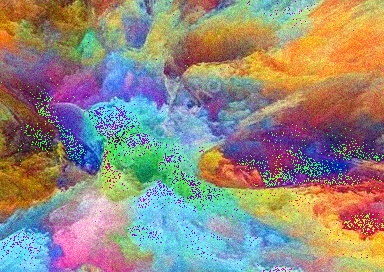
\includegraphics[width=0.5\linewidth]{../output/p0-5-a-2.jpg}
  \caption{Gaussian noise on p0-1-2.jpg green channel}
  \label{fig:sfig1}
\end{subfigure}%
\begin{subfigure}{0.5\textwidth}
  \centering
  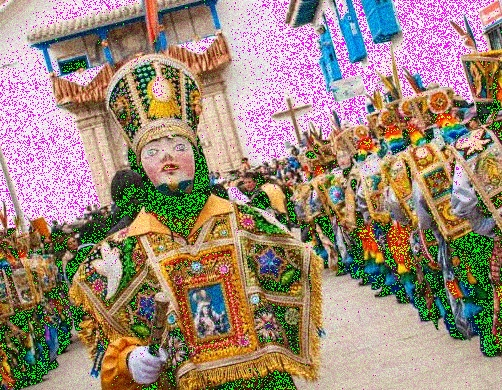
\includegraphics[width=0.5\linewidth]{../output/p0-5-a-3.jpg}
  \caption{Gaussian noise on p0-1-3.jpg green channel}
  \label{fig:sfig2}
\end{subfigure}
\caption{Gaussian noise on green channel}
\label{fig:gaussian-noise-green}
\end{figure}


\item Add the noise using the same sigma to the blue channel instead. Store the output.

The results of adding gaussian noise to the blue channel are shown in figure \ref{fig:gaussian-noise-blue}.

\begin{figure}[h!]
\centering
\begin{subfigure}{0.5\textwidth}
  \centering
  
\includegraphics[width=0.5\linewidth]{../output/p0-5-b-0.jpg}
  \caption{Gaussian noise on p0-1-0.jpg blue channel}
  \label{fig:sfig1}
\end{subfigure}%
\begin{subfigure}{0.5\textwidth}
  \centering
  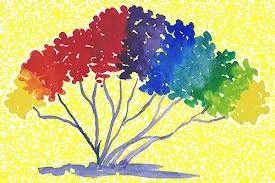
\includegraphics[width=0.5\linewidth]{../output/p0-5-b-1.jpg}
  \caption{Gaussian noise on p0-1-1.jpg blue channel}
  \label{fig:sfig2}
\end{subfigure}
\begin{subfigure}{0.5\textwidth}
  \centering
  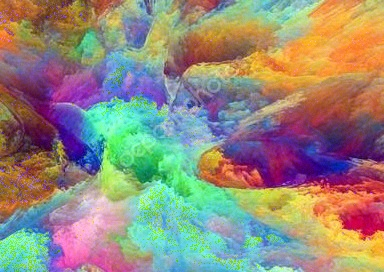
\includegraphics[width=0.5\linewidth]{../output/p0-5-b-2.jpg}
  \caption{Gaussian noise on p0-1-2.jpg blue channel}
  \label{fig:sfig1}
\end{subfigure}%
\begin{subfigure}{0.5\textwidth}
  \centering
  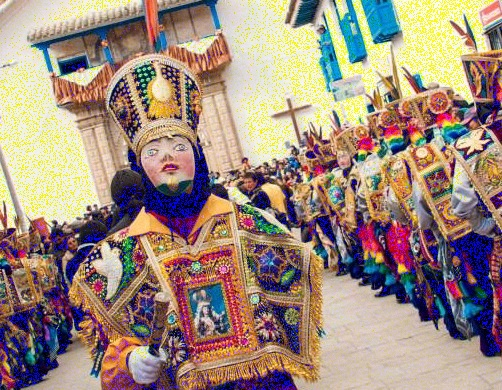
\includegraphics[width=0.5\linewidth]{../output/p0-5-b-3.jpg}
  \caption{Gaussian noise on p0-1-3.jpg blue channel}
  \label{fig:sfig2}
\end{subfigure}
\caption{Gaussian noise on blue channel}
\label{fig:gaussian-noise-blue}
\end{figure}

\item Which image looks better? Why?

The noise in the blue channel looks better because in the final image it generated points of color yellow that do no have a big contrast with the color around them, on the other hand, the noise in the green channel creates purple points that are more notorious.

\end{enumerate}
